%mac
\subsubsection{TÍNH TƯƠNG ĐỐI CỦA CHUYỂN ĐỘNG}
\paragraph{Tính tương đối của quỹ đạo}
\newghichu{Quỹ đạo của chuyển động có tính tương đối, quỹ đạo trong các hệ quy chiếu khác nhau là khác nhau.}
\begin{itemize}
\item Hình vẽ dưới mô tả quỹ đạo của một vật được ném thẳng lên bởi một người A đứng trên xe ô tô đang chuyển động.
\begin{itemize} 
\item Hình (a) là quỹ đạo quan sát bởi người A. 
\item Hình (b) là quỹ đạo quan sát bởi người B đang đứng yên bên đường.
\end{itemize}
\end{itemize}
\centerline{

\includegraphics[width=10cm]{images/ChuyenDongTuongDoi1}	
}
\paragraph{Tính tương đối của vận tốc}
\newghichu{Vận tốc của chuyển động có tính tương đối, vận tốc trong các hệ quy chiếu khác nhau là khác nhau.}
\subsubsection{TỔNG HỢP VẬN TỐC}
\centerline{

\includegraphics[width=8cm]{images/ChuyenDongTuongDoi2}	
}
\begin{itemize}
\item[$\bullet$] Số $1$: ứng với vật chuyển động (thuyền).
\item[$\bullet$] Số $2$: ứng với hệ quy chiếu chuyển động (nước).
\item[$\bullet$] Số $3$: ứng với hệ quy chiếu đứng yên (bờ).
\item[$\bullet$]  $\vec v_{12}$: vận tốc của vật so với hệ quy chiếu chuyển động.
\item[$\bullet$]  $\vec v_{23}$: vận tốc của hệ quy chiếu chuyển động so với hệ quy chiếu đứng yên.
\item[$\bullet$] $\vec v_{13}$: vận tốc của vật so với hệ quy chiếu đứng yên.
\end{itemize}
\begin{itemize}
\item Khi vật $1$ có độ dịch chuyển $\vec d_{12}$ trong hệ quy chiếu chuyển động, đồng thời hệ quy chiếu chuyển động cũng có độ dịch chuyển $\vec d_{23}$ so với hệ quy chiếu đứng yên. Dựa vào phương pháp tọa độ của toán học, ta suy ra biểu thức của độ dịch chuyển tổng hợp:
\begin{align*}
\boder{\vec d_{13}=\vec d_{12}+\vec d_{23}}
\end{align*}
\item Xét trong khoảng thời gian $\Delta t$ rất nhỏ, kết hợp với định nghĩa của vận tốc, ta suy ra biểu thức của vận tốc tổng hợp: 
\begin{align*}
\boder{\vec v_{13}=\vec v_{12}+\vec v_{23}}
\end{align*}
\end{itemize}
\immini{\paragraph{Minh họa về chuyển động cùng phương}
\begin{itemize}
\item Khi thuyền đi xuôi dòng trên sông, nhờ có thêm sự chuyển động cùng chiều của dòng nước nên thuyền sẽ có tốc độ lớn hơn so với khi nước không chảy (trong một hồ nước). Tương tự, khi thuyền đi ngược dòng, vì có thêm sự chuyển động ngược lại của dòng nước nên thuyền sẽ có tốc độ nhỏ hơn khi nước không chảy.
\end{itemize}}{\begin{tikzpicture}[line cap=round, line join=round, scale=1, font=\footnotesize, >=stealth]
\path
(0,0)coordinate(A)
(0,-2)coordinate(B)
;


\draw[blue,->,thick] (0.25,0.25) -- (3,0.25);

\draw[green,->,thick]  (0.25,0.25) -- (2,0.25);

\draw[red,->,thick]  (0.25,-0.25) -- (3,-0.25);

\draw[green,->,thick]  (0.25,-1.75) -- (3,-1.75);

\draw[blue,->,thick]  (3,-2) -- (1,-2);

\draw[red,->,thick]  (0.25,-2.25) -- (1,-2.25);
\node at (1,0.5) {$\vec v_{12}$};
\node at (2.5,0.5) {$\vec v_{23}$};
\node at (1.75,-0.5) {$\vec v_{13}$};
\node at (1.75,-1.5) {$\vec v_{12}$};
\node at (2.25,-2.25) {$\vec v_{23}$};
\node at (0.75,-2.5) {$\vec v_{13}$};

\node at (A) {\faShip};
\node at (B) {\faShip};

\end{tikzpicture}}
\paragraph{Minh họa về chuyển động vuông phương}
\begin{itemize}
\item Một chiếc thuyền máy qua sông với vận tốc có độ lớn $v_{12}$ và hướng vuông góc với dòng sông. Khi nước không chảy thì thuyền sẽ đến bở đối diện ở vị trí $A$.
\item Giả sử rằng, người điều khiển động cơ của thuyền giữ nguyên tốc độ và hướng nhưng nước sông chảy với vận tốc có độ lớn $v_{23}$ và hướng vuông góc với vận tốc của thuyền. Khi đó thuyền sẽ đến bờ đối diện ở vị trí $B$, không trùng với vị trí $A$.
\item Như vậy, khi thuyền đi trong nước sông đang chảy, vận tốc do động cơ của thuyền và vận tốc do nước sông chảy kết hợp với nhau để tạo ra một vận tốc tổng hợp cho thuyền.
\item Vận tốc là một đại lượng vectơ, do đó hai vận tốc có thể được kết hợp bằng phép cộng vectơ theo cùng một cách mà chúng ta đã thấy đối với hai hoặc nhiều độ dịch chuyển.
\end{itemize}
\setcounter{vidu}{0}
\begin{vidu}
\immini[thm]{Một vận động viên bơi về phía Bắc với vận tốc $1,7\ m/s$, nước sông chảy với vận tốc $1,0\ m/s$ về phía Đông. Tìm độ lớn và hướng vận tốc tổng hợp của vận động viên tương tự như với cách tìm độ dịch chuyển tổng hợp.}{\begin{tikzpicture}[line cap=round, line join=round, scale=1, font=\footnotesize, >=stealth,draw=Mapcolor]
\path
(0,0)coordinate(O)
;
\begin{scope}[shift={(0,0)},rotate=0, scale=0.25]
\fill[white] (0,0) -- (2,0) arc[start angle=0, end angle=90, radius=2cm] -- cycle;

\draw[thick,white] (0,0) -- (2,0);
\draw[thick,white] (0,0) -- (0,2);
\draw[thick,white] (2,0) arc[start angle=0, end angle=90, radius=2cm];


\begin{scope}[shift={(0,0)},rotate=90]
\fill[Mapcolor!50] (0,0) -- (2,0) arc[start angle=0, end angle=90, radius=2cm] -- cycle;

\draw[thick,Mapcolor!50] (0,0) -- (2,0);
\draw[thick,Mapcolor!50] (0,0) -- (0,2);
\draw[thick,Mapcolor!50] (2,0) arc[start angle=0, end angle=90, radius=2cm];
\end{scope}

\begin{scope}[shift={(0,0)},rotate=180]
\fill[white] (0,0) -- (2,0) arc[start angle=0, end angle=90, radius=2cm] -- cycle;

\draw[thick,Mapcolor!50] (0,0) -- (2,0);
\draw[thick,white] (0,0) -- (0,2);
\draw[thick,white] (2,0) arc[start angle=0, end angle=90, radius=2cm];
\end{scope}


\begin{scope}[shift={(0,0)},rotate=270]
\fill[Mapcolor!50] (0,0) -- (2,0) arc[start angle=0, end angle=90, radius=2cm] -- cycle;

\draw[thick,Mapcolor!50] (0,0) -- (2,0);
\draw[thick,Mapcolor!50] (0,0) -- (0,2);
\draw[thick,Mapcolor!50] (2,0) arc[start angle=0, end angle=90, radius=2cm];
\end{scope}

\draw (O) circle(2cm);
\draw (O) circle(2.5cm);

\draw (0,2.5) -- (-0.5,2.45) -- (0,4) -- (0,2.5);
\draw[fill=Mapcolor!50] (0,2.5) -- (0.5,2.45) -- (0,4) -- (0,2.5);

\draw (2.5,0) -- (4,0) -- (2.45,0.5) -- (2.5,0);
\draw[fill=Mapcolor!50] (2.5,0) -- (2.45,-0.5) -- (4,0) -- (2.5,0);

\draw (0.5,-2.5) -- (0,-4) -- (0,-2.5) -- (0.5,-2.45);
\draw[fill=Mapcolor!50] (0,-2.5) -- (-0.5,-2.45) -- (0,-4) -- (0,-2.5);


\draw (-2.5,-0.5) -- (-4,0) -- (-2.5,0) -- (-2.45,-0.5);
\draw[fill=Mapcolor!50] (-2.5,0.5) -- (-4,0) -- (-2.5,0) -- (-2.45,0.5);
\end{scope}

\path
(-2,1.5)coordinate(C)
(-4.5,-2.5)coordinate(A)
(-4.5,1.5)coordinate(B)
;

\draw [->,thick, Mapcolor](A)--(B);
\draw [->,thick, Mapcolor](A)--(C);
\draw [->,thick, Mapcolor](B)--(C);

\node at (-5.5,0) {$1,7\ m/s$};
\node at (-2,2) {$1,0\ m/s$};
\node at (-3,-0.5) {$\vec v$};
\node at (-4,-1) {$\theta$};
\draw pic[draw,angle radius=0.8cm]{angle=C--A--B};
\node at (1.5,0) {Đ};
\node at (-1.5,0) {T};
\node at (0,-1.5) {N};
\node at (0,1.5) {B};
\end{tikzpicture}}
\begin{itemize}
\item Vẽ tam giác vectơ.
\begin{itemize}
\item Đặt điểm bắt đầu của vectơ thứ hai ở điểm kết thúc của vectơ đầu tiên.
\item Nối điểm đầu và điểm cuối để thành tam giác vectơ.
\end{itemize}
\item  Tính độ lớn của vectơ tổng hợp: $v=\sqrt{1,7^2+1^2}\approx 1,97\ m/s\approx 2,0\ m/s$.
\item Tính góc $\alpha$ giữa vectơ tổng hợp và vectơ thứ nhất.
\item Do cạnh huyền gần gấp đôi cạnh góc vuông nên góc $\alpha\approx 30^\circ$.
\item Vậy vận tốc tổng hợp của vận động viên xấp xỉ $2,0\ m/s$ và có hướng lệch so với hướng Bắc $30^\circ$ về phía Đông.
\end{itemize}
\end{vidu}
